\documentclass[PhD-Yoann-Dupont.tex]{subfiles}
\begin{document}

Le corpus GENIA \citep{kim2003genia} est un recueil de 2000 articles MEDLINE annotés en entités nommées biomédicales, comprenant plus de 400,000 tokens ainsi que près de 100,000 annotations. Plus généralement, pour effectuer de la reconnaissance d'entités nommées, la variante utilisée est celle du défi JNLPBA 2004 \citep{kim2004introduction}, dont les caractéristiques principales sont données dans le tableau \ref{tab:genia-2004-numbers}. Des exemples d'annotation sont donnés dans la figure\ \ref{fig:genia-examples}.

\begin{table}[ht!]
\centering
\begin{tabular}{|p{0.21\linewidth}|p{0.21\linewidth}|p{0.21\linewidth}|p{0.21\linewidth}|}
\hline
\multicolumn{4}{|c|}{\textbf{corpus Genia}} \\
\hline
\multicolumn{2}{|c|}{\textbf{général}} & \multicolumn{2}{c|}{\textbf{annotations}} \\
\hline
\textbf{type de texte} & articles scientifiques & \textbf{niveaux d'analyse} & $\emptyset$ \\
\hline
\textbf{unités d'analyse} & documents*, phrases & \textbf{structuration} & hiérarchique*,\newline arborescente* \\
\hline
\textbf{volume texte brut} & 3.2 Mo & \textbf{types\newline d'entités} & 5 \\
\hline
\textbf{format} & xml (annotations intégrées) & \textbf{entités\newline inconnues} & 45.25\% \\
\hline
\textbf{langue(s)} & Anglais & \textbf{$\kappa$} & $\emptyset$ \\
\hline
\end{tabular}
\scriptsize{\\ *pour le corpus d'entrainement uniquement}
\caption{Fiche récapitulative du corpus FTB annoté EN}
\label{tab:genia-recap-card}
\end{table}

\begin{table}[ht!]
\centering
\begin{tabular}{|l|cc|}
\cline{2-3}
\multicolumn{1}{l|}{} & train  & test \\
\hline
tokens                & 492551 & 101039 \\
prhases               & 18545  & 3855 \\
entités               & 51301  & 8662 \\
\hline
protein               & 30269  & 5067 \\
DNA                   & 9533   & 1056 \\
RNA                   & 951    & 118 \\
cell line             & 3830   & 500 \\
cell type             & 6718   & 1921 \\
\hline
\end{tabular}
\caption{un aperçu du corpus Genia 2004}
\label{tab:genia-2004-numbers}
\end{table}

\begin{figure}[ht!]
\centering
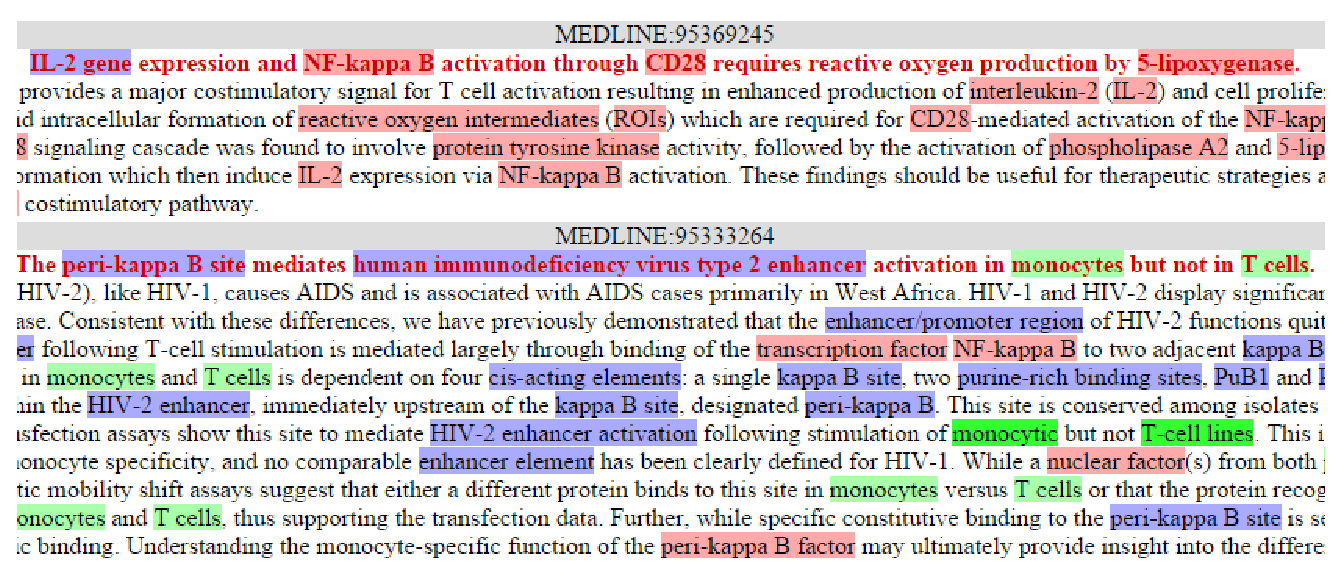
\includegraphics[scale=0.6]{images/genia/examples}
\caption{des exemples d'annotation Genia 2004}
\label{fig:genia-examples}
\end{figure}

Genia dispose de quelques éléments de structuration, mais ces derniers demeurent assez peu nombreux. Un exemple typique est "$[protein]$ gene" $\rightarrow$ "$[DNA]$" (exemple: "IL-2 gene", "IL-2" est une protéine et "IL-2 gene" est un DNA). Genia a également l'inconvénient de ne pas avoir d'accord inter-annotateur malgré la complexité des annotations qu'il propose, sa qualité ne peut donc pas être certifiée. Nous avons cependant pu trouver un document en double dans le corpus, mais annoté par deux annotateurs différents: le document $MEDLINE:97218353$\footnote{cela est noté sur la page de DepGenia: \url{https://files.ifi.uzh.ch/cl/kalju/download/depgenia/v1/} ainsi que par \citet{lease2005parsing}}. Les deux annotations sont données dans la figure\ \ref{fig:genia-medline-97218353}. La tâche sur le corpus Genia dans le défi JNLPBA correspond à reconnaître les entités de plus haut niveau uniquement, nous avons donc évalué les différences entre les deux annotations. Le premier annotateur a donné 11 entités contre 17 pour le second. Parmi toutes les annotations, 10 étaient en commun pour les deux annotateurs, 1 avait une différence de frontière et 6 présentes chez uniquement un des deux annotateurs. Bien que statistiquement non significatif, ces différences illustrent l'incertitude quant à la qualité du corpus.

\begin{figure}[ht!]
\centering
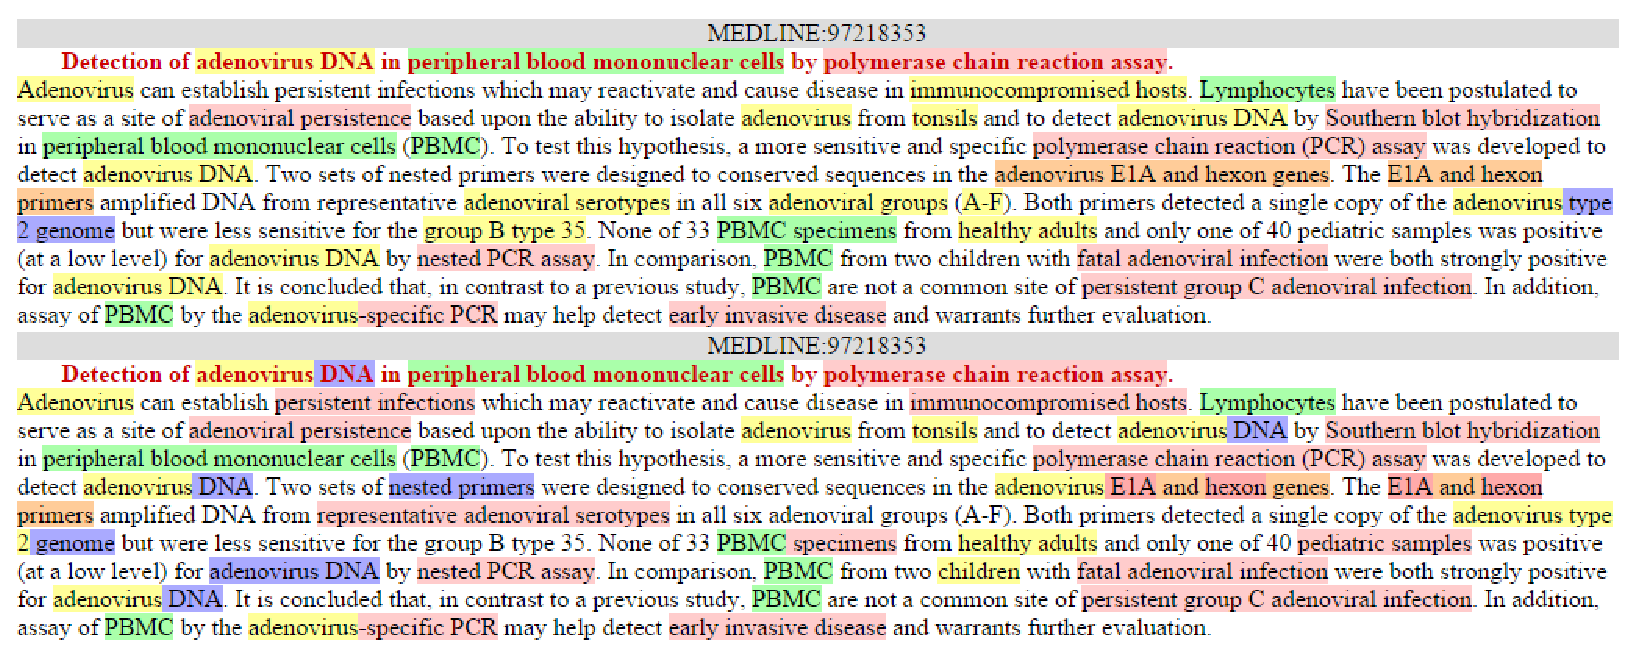
\includegraphics[scale=0.5]{images/genia/MEDLINE-97218353}
\caption{comparaison des annotations sur le document MEDLINE:97218353}
\label{fig:genia-medline-97218353}
\end{figure}

\end{document}